\ifdefined\iscombined
	\quiz{Quiz 1}
\else
\documentclass{article}
\usepackage{xparse}
\usepackage{tabularx}
\usepackage{changepage}
\usepackage{listings}
\usepackage{amsthm}
\usepackage{comment}
\usepackage{amsmath}
\usepackage{braket}
\usepackage{amsfonts}
\usepackage{amssymb}
\usepackage{sectsty}
\usepackage{hyperref}
\usepackage{fancyhdr}
\usepackage[top=1in,bottom=1in,left=1in,right=1in]{geometry}
\usepackage{float}
\usepackage{graphicx}
\usepackage{mathtools}
\usepackage{tikz}
\usetikzlibrary{arrows, arrows.meta}

\date{
	\vspace{-.75em}
	{\large \today}
}

\title{
	\vspace*{-1.5em}
	{\Huge Quiz 1} \\
	\vspace{-1em}
	\rule{\textwidth/2}{.01em} \\
	\vspace{-.75em}
}

\author{
	{\large Matthew Farah}
}

\hypersetup{
	colorlinks=true,
	linkcolor=blue,
	filecolor=magenta,
	urlcolor=blue,
	citecolor=blue,
	anchorcolor=blue
}

\fancyhead{}
\fancyhead[L]{\today}
\fancyhead[R]{Quiz 1}

\setlength{\parindent}{0cm}

\tikzset{vertex/.style = {shape = circle, draw, minimum size = 2em}}
\tikzset{edge/.style = {-,> = latex'}}

\newenvironment{solution}{
	\vspace{.5em}
	\par
	\begin{adjustwidth}{1.5em}{}
	\textbf{{Solution:}}
	\par
	\vspace{.5em}
}{
	\vspace{1em}
	\end{adjustwidth}
	\setcounter{step}{0}
}

\makeatother
\makeatletter

\newcounter{step}
\renewcommand{\thestep}{\Roman{step}}

\newenvironment{step}{
	\refstepcounter{step}
	\vspace{1em}\par\noindent
	\ignorespaces\noindent\textbf{(\thestep)}
	\ignorespaces
}{
	\par
	\vspace{1.5em}
}

\newcounter{problem}
\renewcommand{\theproblem}{\arabic{problem}}

\newenvironment{problem}[1][]{
	\newpage
	\refstepcounter{problem}
	\setcounter{subproblem}{0}
	\vspace{.5em}\par\noindent
	\begin{adjustwidth}{1.5em}{}
	\noindent\textbf{Problem \theproblem: }\noindent\textit{#1}
	\par
	\phantomsection
	\addcontentsline{toc}{section}{\protect{\large{Problem \theproblem}}}
}{
	\vspace{.5em}
	\end{adjustwidth}
}

\newcounter{subproblem}
\renewcommand{\thesubproblem}{\alph{subproblem}}

\newenvironment{subproblem}{
	\setcounter{step}{0}
	\refstepcounter{subproblem}
	\phantomsection
	\addcontentsline{toc}{subsection}{\protect{\large{(\thesubproblem)}}}
	\begin{adjustwidth}{1.5em}{}
	\noindent{\textbf{(\thesubproblem) }}\ignorespaces
}{
	\par
	\vspace{.5em}
	\end{adjustwidth}
}

\newcounter{lemma}
\renewcommand{\thelemma}{\arabic{lemma}}

\newenvironment{lemma}[1][]{
	\refstepcounter{lemma}
	\vspace{1em}\par\noindent
	\noindent\textbf{Lemma ({#1}): }\noindent\ignorespaces
}{
	\vspace{.5em}
}

\newcounter{proposition}
\renewcommand{\theproposition}{\arabic{proposition}}

\newenvironment{proposition}{
	\refstepcounter{proposition}
	\vspace{1em}\par\noindent
	\noindent\textbf{Proposition:}
	\noindent\textit
	\ignorespaces
}{
	\vspace{.5em}
}

\newcommand{\supp}[1]{\text{supp}({#1})}
\newcommand{\ord}[1]{\text{ord}({#1})}
\newcommand{\gen}[1]{\langle {#1} \rangle}
\newcommand{\lcm}[2]{\text{lcm}({#1}, {#2})}

\renewcommand{\mod}[1]{\ (\text{mod} \; {#1})}

\sectionfont{\fontsize{12}{12}\bfseries}
\subsectionfont{\fontsize{10}{12}\normalfont}
\subsubsectionfont{\fontsize{10}{12}\normalfont}

\begin{document}

\maketitle
\pagestyle{fancy}

\newcolumntype{Y}{>{\centering\arraybackslash}X}

\tableofcontents

\fi

\newpage

Please note the quiz is based on the following topics:
\begin{itemize}
	\item The group axioms.
	\item Permutations.
	\item Subgroups.
\end{itemize}

\begin{problem}
	Fill in the blanks of each sentence to make them correct. For each, let $A$ and $B$ be two sets, and let $f \colon A \rightarrow B$ be a function.
\end{problem}

\begin{subproblem}
	$f$ is injective if: \underline{\hspace{2em}} $a_1, a_2 \in A$, \underline{\hspace{2em}} $f(a_1) = f(a_2)$, \underline{\hspace{2em}} $a_1 = a_2$.
\end{subproblem}

\begin{solution}
	$f$ is injective if: \underline{for all} $a_1, a_2 \in A$, \underline{if} $f(a_1) = f(a_2)$, \underline{then} $a_1 = a_2$.
\end{solution}

\begin{subproblem}
	$f$ is surjective if: \underline{\hspace{2em}} $b \in B$, \underline{\hspace{2em}} $a \in A$ \underline{\hspace{2em}} $f(a) = b$.
\end{subproblem}

\begin{solution}
	$f$ is surjective if: \underline{for all} $b \in B$, \underline{there exists} $a \in A$ \underline{such that} $f(a) = b$.
\end{solution}

\begin{problem}
	What are all the units modulo 10?
\end{problem}

\begin{solution}
	Recall than an integer $u \in \mathbb{Z}_{10}$ is a unit modulo 10 if there exists some other integer $v \in \mathbb{Z}_{10}$ such that $uv \equiv 1 \mod{n}$. \\

	By Proposition 1.7, we know that an integer $u$ is a unit modulo $n$ if and only if $\gcd(u, n) = 1$, and since:

	\vspace{2em}
	
	\begin{tabularx}{\linewidth}{Y Y}
		$\gcd(0, 10) = 10$ & $\gcd(5, 10) = 5$ \\
		$\boxed{\gcd(1, 10) = 1}$ & $\gcd(6, 10) = 2$ \\
		$\gcd(2, 10) = 2$ & $\boxed{\gcd(7, 10) = 1}$ \\
		$\boxed{\gcd(3, 10) = 1}$ & $\gcd(8, 10) = 2$ \\
		$\gcd(4, 10) = 2$ & $\boxed{\gcd(9, 10) = 1}$ \\
	\end{tabularx}

	\vspace{2em}

	We have that $1, 3, 7, and 9$ are all the units modulo $10$ (and hence $\mathbb{Z}^{\times}_{10} = \set{1, 3, 7, 9}$).
\end{solution}

\begin{problem}
	What is the cycle type of each of the following permutations? Assume all permutations belong to the group $S_7$.
\end{problem}

\begin{subproblem}
	$(15)(27)$
\end{subproblem}

\begin{solution}
	Since there are are clearly two cycles of length two each present in this permutation, its cycle type must be:

	\begin{gather*}
		(2, 2, 1, 1, 1) \\
	\end{gather*}

	Since $3, 4$, and $6$ must all be fixed points of the permutation.
\end{solution}

\begin{subproblem}
	$(15)(374)(26)$
\end{subproblem}

\begin{solution}
	As before, there are two cycles of length two each in the given permutation, however this time there is also a single cycle of length three. Arranged in order, these lengths mean that the cycle type of the permutation above is:

	\begin{gather*}
		(3, 2, 2)
	\end{gather*}
\end{solution}

\begin{subproblem}
	$(23)(345)$
\end{subproblem}

\begin{solution}
	Don't let this permutation mislead you! Although at first glance, the permutation above appears to have two cycles of lengths two and three respectively, this is because the permutation above is actually the composition of two different permutations. Since these two permutations do not have an empty intersection of their supports, we can (and should) infer that this permutation can be simplified down first! And indeed we find that:

	\begin{align*}
		(23)(345) &= (2345) \\
	\end{align*}

	Thus giving us a cycle type of:

	\begin{gather*}
		(4, 1, 1, 1) \\
	\end{gather*}

	for our permtation.
\end{solution}

\begin{subproblem}
	$(321)$
\end{subproblem}

\begin{solution}
	Lastly, this permutation just clearly and simply has a cycle type of:

	\begin{gather*}
		(3, 1, 1, 1, 1)
	\end{gather*}
\end{solution}

\begin{problem}
	Let $\sigma = (153)(24)$ and $\tau = (4135)$. What is $\sigma\tau$?
\end{problem}

\begin{solution}
	We know that $\sigma\tau$ is a way of expressing the permutation composition $\sigma(\tau(a))$, where $a \in \set{1, 2, 3, 4, 5}$. By the given definitions of $\sigma$ and $\tau$, we know that:

	\begin{align*}
		\sigma(\tau(1)) &= \sigma(3) &= 1 \\
		\sigma(\tau(2)) &= \sigma(2) &= 4 \\
		\sigma(\tau(3)) &= \sigma(5) &= 3 \\
		\sigma(\tau(4)) &= \sigma(1) &= 5 \\
		\sigma(\tau(5)) &= \sigma(4) &= 2 \\
	\end{align*}

	Therefore, $\sigma\tau$ permutes the elements of $\set{1, 2, 3, 4, 5}$ in the following way:

	\begin{gather*}
		1 \rightarrow 1 \\
		2 \rightarrow 4 \rightarrow 5 \rightarrow 2 \\
		3 \rightarrow 3 \\
	\end{gather*}

	Giving us that:

	\begin{align*}
		\sigma\tau = (245)
	\end{align*}
\end{solution}

\begin{problem}
	Determine whether each of the following permutations are even or odd.
\end{problem}

\begin{subproblem}
	$(12)(34)$
\end{subproblem}

\begin{solution}
	This permutation is indeed even. Without taking the time to calculate the determinant of its corresponding permutation matrix, we can instead rely on the fact: \\

	``A permutation is even if and only if it can be expressed as the composition of an even number of permutations of length two''. \\

	Although I won't prove the theorem above, I will make use of it repeatedly so just trust me bro. \\

	Anyways, since the permutation $(12)(34)$ is clearly composed of two cycles of length two, we know that the permutation must be even.
\end{solution}

\begin{subproblem}
	$(1234)$
\end{subproblem}

\begin{solution}
	This permutation, on the other hand is odd. Attempting to decompose the permutation into cycles of length two, we find that:

	\begin{align*}
		(1234) &= (12)(23)(34) \\
	\end{align*}

	And so, since this is an odd number of length two cycles, the permutation is necessarily odd.
\end{solution}

\begin{subproblem}
	$(123)(456)$
\end{subproblem}

\begin{solution}
	Using the same approach as before, since:

	\begin{align*}
		(123)(456) &= (12)(23)(45)(56) \\
	\end{align*}

	We know that $(123)(456)$ is expressible as the composition of four cycles of length two, which is an even number of cycles! So $(123)(456)$ is indeed even.
\end{solution}

\begin{subproblem}
	Any permutation of cycle type $(5, 4, 2, 1)$.
\end{subproblem}

\begin{solution}
	A little tricker this time, but taking $(abcde)(fghi)(jk)$ to be an arbitrary permutation of cycle type $(5, 4, 2, 1)$, we can see that because:

	\begin{align*}
		(abcde)(fghi)(jk) &= \underbrace{(ab)}_{1}\,
		\underbrace{(bc)}_{2}\,
		\underbrace{(cd)}_{3}\,
		\underbrace{(de)}_{4}\,
		\underbrace{(fg)}_{5}\,
		\underbrace{(gh)}_{6}\,
		\underbrace{(hi)}_{7}\,
		\underbrace{(jk)}_{8} \\
	\end{align*}

	Any permutation of cycle type $(5, 4, 2, 1)$ must be even.
\end{solution}

\begin{problem}
	Which of the following statements are true?
\end{problem}

\begin{subproblem}
	$D_{4}$ is a subgroup of $A_{4}$.
\end{subproblem}

\begin{solution}
	This statement is false, which I will show by a simple counter example.

	Consider the permutation $(1234)$. We know $(1234)$ belongs to $D_4$ since it corresponds to a clockwise rotation of a square, which is adjacency preserving. In case you're not convinced, we can see graphically that the vertices of a square are permuted by $(1234)$ from:

	
	\vspace{2em}

	\begin{center}
		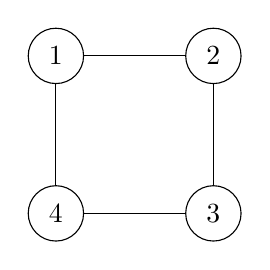
\begin{tikzpicture}
			\node[vertex] (a) at (0, 2) {$1$};
			\node[vertex] (b) at (2, 2) {$2$};
			\node[vertex] (c) at (2, 0) {$3$};
			\node[vertex] (d) at (0, 0) {$4$};

			\draw[edge] (a) to (b);
			\draw[edge] (b) to (c);
			\draw[edge] (c) to (d);
			\draw[edge] (d) to (a);
		\end{tikzpicture}
	\end{center}

	\vspace{2em}
	
	to:

	\vspace{2em}

	\begin{center}
		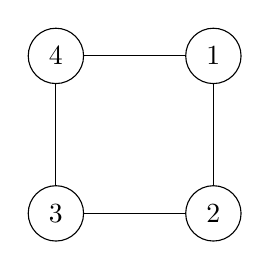
\begin{tikzpicture}
			\node[vertex] (a) at (0, 2) {$4$};
			\node[vertex] (b) at (2, 2) {$1$};
			\node[vertex] (c) at (2, 0) {$2$};
			\node[vertex] (d) at (0, 0) {$3$};

			\draw[edge] (a) to (b);
			\draw[edge] (b) to (c);
			\draw[edge] (c) to (d);
			\draw[edge] (d) to (a);
		\end{tikzpicture}
	\end{center}

	\vspace{2em}

	And hence, $(1234) \in D_{4}$. However, decomposing $(1234)$ into length two cycles, we have that:

	\begin{align*}
		(1234) &= (12)(23)(34) \\
	\end{align*}

	Meaning $(1234)$ is an odd permutation (we actually already concluded this earlier by the result of \textbf{Problem 5 (a)}). \\

	So, because $A_{4}$ is definitionally the set of all even permutations in $S_{4}$, $(1234)$ cannot belong to $A_4$. Thus, since there exists an element in $D_{4}$ not belonging to $A_{4}$, $D_{4}$ cannot be a subset of $A_{4}$.
\end{solution}

\begin{subproblem}
	$D_{4}$ is a subgroup of $S_{4}$.
\end{subproblem}

\begin{solution}
	This statement is true, and follows trivially from the definition of $D_{4}$ as the subset of all adjacency preserving permutations in $S_{4}$.
\end{solution}

\begin{subproblem}
	$\set{1, 3, 5}$ is a subgroup of $\mathbb{Z}_{6}$.
\end{subproblem}

\begin{solution}
	This statement is false. \\

	To see why, recall that any subgroup must be closed under its parent group's binary operation. However, despite the fact that both $1$ and $3$ both belong to $\mathbb{Z}_{6}$, it isn't the case that $(1 + 3) \mod{6} \equiv 4 \mod{6} \equiv 4$ belongs to $\set{1, 3, 5}$. \\

	Thus, since $\set{1, 3, 5}$ isn't closed under addition modulo $6$, $\set{1, 3, 5}$ cannot be a subgroup of $\mathbb{Z}_{6}$.
\end{solution}

\begin{subproblem}
	$\set{0, 3, 6}$ is a subgroup of $\mathbb{Z}_{9}$.
\end{subproblem}

\begin{solution}
	This statement is true. \\

	To see why, we can recall that for $\set{0, 3, 6}$ to be a subgroup of $\mathbb{Z}_{9}$, it must satisfy the following criteria:
	\begin{enumerate}
		\item $\set{0, 3, 6}$ must be closed under $\mathbb{Z}_{9}$'s binary operator.
		\item $\set{0, 3, 6}$ must contain $\mathbb{Z}_{9}$'s identity element.
		\item Every element in $\set{0, 3, 6}$ must have an inverse also in $\set{0, 3, 6}$. \\
	\end{enumerate}

	So, we can show that $\set{0, 3, 6}$ is a subgroup of $\mathbb{Z}_{9}$ by proving:

	\begin{step}
		$\set{0, 3, 6}$ is closed under addition modulo $9$.
	\end{step}

	Since $\set{0, 3, 6}$'s Cayley table looks like this:

	\vspace{2em}

	\begin{tabularx}{\linewidth}{Y || Y | Y | Y}
		$ + \mod{9}$ & 0 & 3 & 6 \\
		\hline
		\hline
		0 & 0 & 3 & 6 \\
		\hline
		3 & 3 & 6 & 0 \\
		\hline
		6 & 6 & 0 & 3 \\
	\end{tabularx}
	
	\vspace{2em}

	We can easily see that $\set{0, 3, 6}$ is indeed closed under addition modulo 9.

	\begin{step}
		$\set{0, 3, 6}$ contains $\mathbb{Z}_{9}$'s identity element.
	\end{step}

	Recalling that the identity of $\mathbb{Z}_{9}$ under addition modulo 9 is 0, we can trivially that since $0 \in \set{0, 3, 6}$ as well, $\set{0, 3, 6}$ also contains $\mathbb{Z}_{9}$'s identity element.

	\begin{step}
		Every element in $\set{0, 3, 6}$ has an inverse under addition modulo $9$ in $\set{0, 3, 6}$.
	\end{step}

	Deferring to the Cayley table constructed in step \textbf{(I)}, we can see that since:

	\begin{align*}
		(0 + 0) \mod{9} &\equiv (0 + 0) \mod{9} &&\equiv 0 \\
		(3 + 6) \mod{9} &\equiv (6 + 3) \mod{9} &&\equiv 0 \\
		(6 + 3) \mod{9} &\equiv (3 + 6) \mod{9} &&\equiv 0 \\
	\end{align*}

	and $0$ is the identity element, $\set{0, 3, 6}$ is closed under inverses. \\

	And so, because \textbf{(I)}, \textbf{(II)}, and \textbf{(III)} all hold, we can thus conclude $\set{0, 3, 6}$ is indeed a subgroup of $\mathbb{Z}_{9}$
\end{solution}

\begin{subproblem}
	$\set{(), (123), (132)}$ is a subgroup of $S_{5}$.
\end{subproblem}

\begin{solution}
	This statement is also true! \\

	So as not to belabour the point, I will simply state that since the Cayley table for $\set{(), (123), (132)}$ looks like:

	\vspace{2em}

	\begin{tabularx}{\linewidth}{Y || Y | Y | Y}
		$\circ$ & $()$ & $(123)$ & $(132)$ \\
		\hline
		\hline
		$()$ & $()$ & $(123)$ & $(132)$ \\
		\hline
		$(123)$ & $(123)$ & $(132)$ & $()$ \\
		\hline
		$(132)$ & $(132)$ & $()$ & $(123)$ \\
	\end{tabularx}

	\vspace{2em}

	It very easily must follow that $\set{(), (123), (132)}$ is a subgroup of $S_{6}$.
\end{solution}

\begin{subproblem}
	The set of diagonal $2 \times 2$ matrices is a subgroup of $GL_{2}(\mathbb{R})$.
\end{subproblem}

\begin{solution}
	This statement is false! \\

	The reason why is actually deceptively obvious. Since the matrix:

	\begin{gather*}
		\begin{pmatrix}
			0 & 0 \\
			0 & 0
		\end{pmatrix} \\
	\end{gather*}

	is indeed a diagonal $2 \times 2$ matrix, it would belong to such a proposed subgroup. Yet, taking the determinant, we have that:

	\begin{align*}
		\det{\begin{pmatrix}
			0 & 0 \\
			0 & 0
		\end{pmatrix}} &= (0)(0) - (0)(0) \\
		&= 0 \\
	\end{align*}

	And since $GL_{2}(\mathbb{R})$ is the set of all $2 \times 2$ matrices with a non-zero determinant, $\begin{pmatrix} 0 & 0 \\ 0 & 0 \end{pmatrix} \not\in GL_{2}(\mathbb{R})$. \\

	Thus, since any such set would fail to even be a subset of $GL_{2}(\mathbb{R})$, it immediately follows that it cannot be a subgroup of $GL_{2}(\mathbb{R})$ as well.
\end{solution}

\begin{problem}
	The order of a group $G$ is the number of elements it has and is denoted by $|G|$. What is the order of each of the following groups?
\end{problem}

\begin{subproblem}
	$D_{4}$.
\end{subproblem}

\begin{solution}
	The order of $D_{4}$ is 8 since $D_{n}$ always contains $2n$-many permutations ($n$-many rotations and $n$-many reflections respectively) and so:

	\begin{align*}
		|D_{4}| &= (2)(4) \\
		&= 8
	\end{align*}
\end{solution}

\begin{subproblem}
	$S_{5}$.
\end{subproblem}

\begin{solution}
	The order of $S_{5}$ is 120 since $S_{n}$ always has $n!$-many permutations (because $S_{n}$ is definitionally the set of all permutations of $\set{1, \ldots, n}$) and so:

	\begin{align*}
		|S_{5}| &=  5! \\
		&= (5)(4)(3)(2)(1) \\
		&= 120
	\end{align*}
\end{solution}

\begin{subproblem}
	$A_{5}$.
\end{subproblem}

\begin{solution}
	The order of $A_{5}$ is 60 because $A_{n}$ always has $\frac{n!}{2}$-many permutations (since $A_{n}$ is definitionally the set of all even permutations in $S_{n}$, and exactly half of the permutations in $S_{n}$ are odd) and so:

	\begin{align*}
		|A_{5}| &= \frac{5!}{2} \\
		&= \frac{120}{2} \\
		&= 60
	\end{align*}
\end{solution}

\begin{subproblem}
	$\mathbb{Z}_{15}$.
\end{subproblem}

\begin{solution}
	The order $\mathbb{Z}_{15}$ is 15 because trivially $\mathbb{Z}_{15} = \set{0, 1, 2, 3, 4, 5, 6, 7, 8, 9, 10, 11, 12, 13, 14}$.
\end{solution}

\begin{subproblem}
	$\mathbb{Z}^{\times}_{15}$.
\end{subproblem}

\begin{solution}
	The order of $\mathbb{Z}^{\times}_{15}$ is 8 because $\mathbb{Z}^{\times}_{15}$ is the set of all units modulo $15$, and since:

	\vspace{2em}

	\begin{tabularx}{\linewidth}{Y Y Y}
		$\gcd(0, 15) = 15$ & $\gcd(5, 15) = 5$ & $\gcd(10, 15) = 5$ \\[4pt]
		$\boxed{\gcd(1, 15) = 1}$ & $\gcd(6, 15) = 3$ & $\boxed{\gcd(11, 15) = 1}$ \\[4pt]
		$\boxed{\gcd(2, 15) = 1}$ & $\boxed{\gcd(7, 15) = 1}$ & $\gcd(12, 15) = 3$ \\[4pt]
		$\gcd(3, 15) = 3$ & $\gcd(8, 15) = 1$ & $\boxed{\gcd(13, 15) = 1}$ \\[4pt]
		$\boxed{\gcd(4, 15) = 1}$ & $\gcd(9, 15) = 3$ & $\boxed{\gcd(14, 15) = 1}$ \\[4pt]
	\end{tabularx}

	\vspace{2em}

	we can conclusively state both that $\mathbb{Z}^{\times}_{15} = \set{1, 2, 4, 7, 8, 11, 13, 14}$ and $|\mathbb{Z}^{\times}_{15}| = 8$, since an element $u \in \mathbb{Z}^{\times}_{15}$ is a unit modulo 15 if and only if $\gcd(u, 15) = 1$.
\end{solution}

\begin{problem}
	What is the inverse of each of the following elements, in their respective groups?
\end{problem}

\begin{subproblem}
	42, in the group $\mathbb{Z}_{65}$.
\end{subproblem}

\begin{solution}
	The inverse of 42 in $\mathbb{Z}_{65}$ is 23, since:

	\begin{align*}
		\boxed{(42 + 23)} \mod{65} &\equiv 65 \mod{65} \\
		&\equiv \boxed{0} \\
		&\equiv 65 \mod{65} \\
		&\equiv \boxed{(23 + 42)} \mod{65}
	\end{align*}
\end{solution}

\begin{subproblem}
	3, in the group $\mathbb{Z}^{\times}_{50}$.
\end{subproblem}

\begin{solution}
	The inverse of 3 in $\mathbb{Z}^{\times}_{50}$ is 17, since:

	\begin{align*}
		\boxed{(3)(17)} \mod{50} &\equiv 51 \mod{50} \\
		&\equiv \boxed{1} \\
		&\equiv 51 \mod{50} \\
		&\equiv \boxed{(17)(3)} \mod{50}
	\end{align*}
\end{solution}

\begin{subproblem}
	$(2, 7)$, in the group $\mathbb{Z}^{\times}_{5} \times \mathbb{Z}_{10}$
\end{subproblem}

\begin{solution}
	The inverse of $(2, 7)$ in $\mathbb{Z}^{\times}_{5} \times \mathbb{Z}_{10}$ is (3, 3), since:

	\begin{align*}
		\boxed{(2, 7)(3, 3)} &= ((2)(3) \mod{5}, (7 + 3) \mod{10}) \\
		&\equiv (6 \mod{5}, 10 \mod{10}) \\
		&\equiv (1, 0) \\
		&\equiv (6 \mod{5}, 10 \mod{10}) \\
		&\equiv ((3)(2) \mod{5}, (3 + 7) \mod{10}) \\
		&= \boxed{(2, 7)(3, 3)} \\
	\end{align*}
\end{solution}

\begin{problem}
	Which of the following permutations is an element of $D_{5}$?
\end{problem}

\begin{subproblem}
	$(25)(34)$.
\end{subproblem}

\begin{solution}
	$(25)(34)$ does belong to $D_{5}$. \\

	For this and each of the following problems, we will determine if the given permutation belongs to $D_{5}$ by performing the permutation on the following pentagon:

	\vspace{2em}

	\begin{center}
		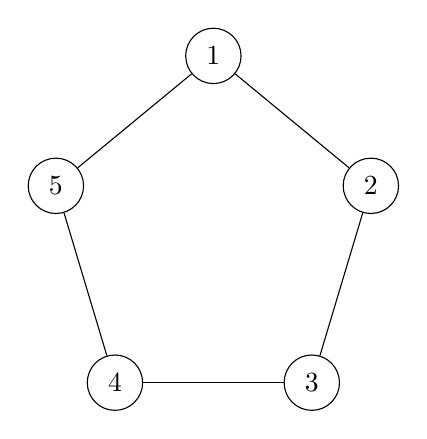
\begin{tikzpicture}
			\node[vertex] (a) at (2, 4.9) {$1$};
			\node[vertex] (b) at (4, 3.25) {$2$};
			\node[vertex] (c) at (3.25, 0.75) {$3$};
			\node[vertex] (d) at (0.75, 0.75) {$4$};
			\node[vertex] (e) at (0, 3.25) {$5$};

			\draw[edge] (a) to (b);
			\draw[edge] (b) to (c);
			\draw[edge] (c) to (d);
			\draw[edge] (d) to (e);
			\draw[edge] (e) to (a);
		\end{tikzpicture}
	\end{center}

	\vspace{2em}

	and checking if adjacency was indeed preserved. Now, in the case of the permutation $(25)(34)$, since the resultant pentagon looks like:

	\vspace{2em}

	\begin{center}
		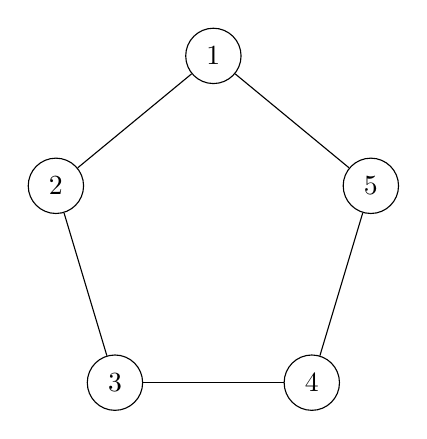
\begin{tikzpicture}
			\node[vertex] (a) at (2, 4.9) {$1$};
			\node[vertex] (b) at (4, 3.25) {$5$};
			\node[vertex] (c) at (3.25, 0.75) {$4$};
			\node[vertex] (d) at (0.75, 0.75) {$3$};
			\node[vertex] (e) at (0, 3.25) {$2$};

			\draw[edge] (a) to (b);
			\draw[edge] (b) to (c);
			\draw[edge] (c) to (d);
			\draw[edge] (d) to (e);
			\draw[edge] (e) to (a);
		\end{tikzpicture}
	\end{center}

	\vspace{2em}

	the permutation is clearly adjacency-preserving and hence, $(25)(34) \in D_{5}$.
\end{solution}

\begin{subproblem}
	$(12)(35)$.
\end{subproblem}

\begin{solution}
	$(12)(35)$ does belong to $D_{5}$, since permuting the base pentagon by $(12)(35)$ looks like:
	
	\vspace{2em}

	\begin{minipage}{0.40\textwidth}
		\begin{center}
			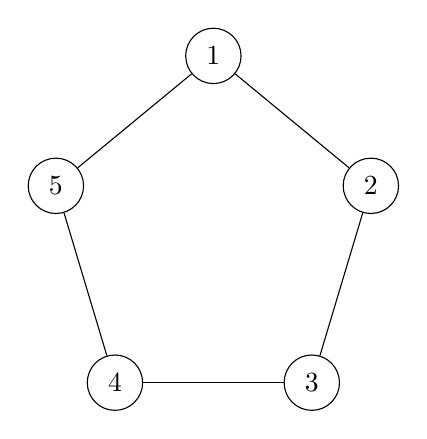
\begin{tikzpicture}
				\node[vertex] (a) at (2, 4.9) {$1$};
				\node[vertex] (b) at (4, 3.25) {$2$};
				\node[vertex] (c) at (3.25, 0.75) {$3$};
				\node[vertex] (d) at (0.75, 0.75) {$4$};
				\node[vertex] (e) at (0, 3.25) {$5$};
	
				\draw[edge] (a) to (b);
				\draw[edge] (b) to (c);
				\draw[edge] (c) to (d);
				\draw[edge] (d) to (e);
				\draw[edge] (e) to (a);
			\end{tikzpicture}
		\end{center}
	\end{minipage}
	\begin{minipage}{0.04\textwidth}
		\begin{center}
			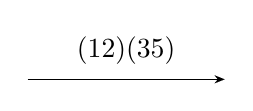
\begin{tikzpicture}
				\draw[-{Stealth[length=1.25mm, width=1mm]}, line width=0.01pt] (0,0) -- (2.5,0)
				node[midway, above=2pt] {$(12)(35)$};
			\end{tikzpicture}
		\end{center}
	\end{minipage}
	\begin{minipage}{0.56\textwidth}
		\begin{center}
			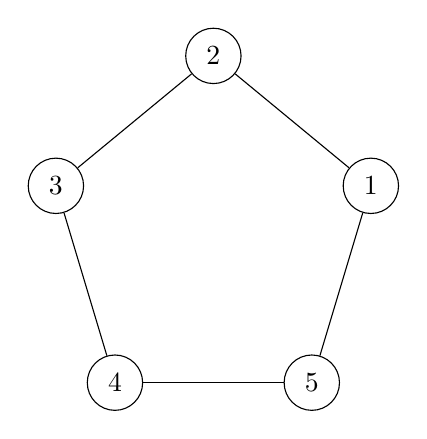
\begin{tikzpicture}
				\node[vertex] (a) at (2, 4.9) {$2$};
				\node[vertex] (b) at (4, 3.25) {$1$};
				\node[vertex] (c) at (3.25, 0.75) {$5$};
				\node[vertex] (d) at (0.75, 0.75) {$4$};
				\node[vertex] (e) at (0, 3.25) {$3$};

				\draw[edge] (a) to (b);
				\draw[edge] (b) to (c);
				\draw[edge] (c) to (d);
				\draw[edge] (d) to (e);
				\draw[edge] (e) to (a);
			\end{tikzpicture}
		\end{center}
	\end{minipage}

	\vspace{2em}

	which is evidently adjacency-preserving. Thus, $(12)(35) \in D_{5}$.
\end{solution}

\begin{subproblem}
	$(13)(24)$.
\end{subproblem}

\begin{solution}
	$(13)(24)$ doesn't belong to $D_{5}$. To see why, notice that $(13)(24)$ would permute the vertices of a pentagon like so:

	\vspace{2em}

	\begin{minipage}{0.40\textwidth}
		\begin{center}
			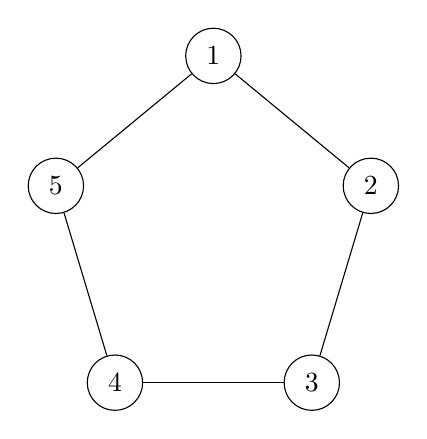
\begin{tikzpicture}
				\node[vertex] (a) at (2, 4.9) {$1$};
				\node[vertex] (b) at (4, 3.25) {$2$};
				\node[vertex] (c) at (3.25, 0.75) {$3$};
				\node[vertex] (d) at (0.75, 0.75) {$4$};
				\node[vertex] (e) at (0, 3.25) {$5$};
	
				\draw[edge] (a) to (b);
				\draw[edge] (b) to (c);
				\draw[edge] (c) to (d);
				\draw[edge] (d) to (e);
				\draw[edge] (e) to (a);
			\end{tikzpicture}
		\end{center}
	\end{minipage}
	\begin{minipage}{0.04\textwidth}
		\begin{center}
			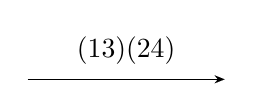
\begin{tikzpicture}
				\draw[-{Stealth[length=1.25mm, width=1mm]}, line width=0.01pt] (0,0) -- (2.5,0)
				node[midway, above=2pt] {$(13)(24)$};
			\end{tikzpicture}
		\end{center}
	\end{minipage}
	\begin{minipage}{0.56\textwidth}
		\begin{center}
			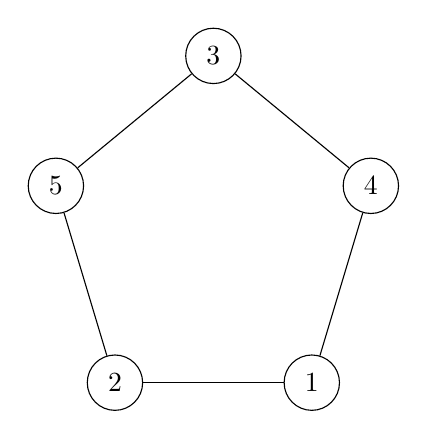
\begin{tikzpicture}
				\node[vertex] (a) at (2, 4.9) {$3$};
				\node[vertex] (b) at (4, 3.25) {$4$};
				\node[vertex] (c) at (3.25, 0.75) {$1$};
				\node[vertex] (d) at (0.75, 0.75) {$2$};
				\node[vertex] (e) at (0, 3.25) {$5$};

				\draw[edge] (a) to (b);
				\draw[edge] (b) to (c);
				\draw[edge] (c) to (d);
				\draw[edge] (d) to (e);
				\draw[edge] (e) to (a);
			\end{tikzpicture}
		\end{center}
	\end{minipage}

	\vspace{2em}

	which isn't adjacency preserving since, for example, $1$ becomes adjacent to vertex $4$ after the permutation, whereas that was not the case in the original pentagon. Thus, since $(13)(24)$ isn't an adjacency preserving permutation, it cannot belong to $D_{5}$.
\end{solution}

\begin{subproblem}
	$(14)(23)$.
\end{subproblem}

\begin{solution}
	$(14)(23)$ does belong to $D_{5}$, since permuting the base pentagon by $(14)(23)$ looks like:

	\vspace{2em}
	
	\begin{minipage}{0.40\textwidth}
		\begin{center}
			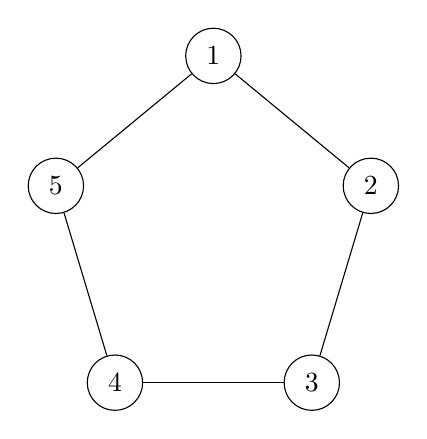
\begin{tikzpicture}
				\node[vertex] (a) at (2, 4.9) {$1$};
				\node[vertex] (b) at (4, 3.25) {$2$};
				\node[vertex] (c) at (3.25, 0.75) {$3$};
				\node[vertex] (d) at (0.75, 0.75) {$4$};
				\node[vertex] (e) at (0, 3.25) {$5$};
	
				\draw[edge] (a) to (b);
				\draw[edge] (b) to (c);
				\draw[edge] (c) to (d);
				\draw[edge] (d) to (e);
				\draw[edge] (e) to (a);
			\end{tikzpicture}
		\end{center}
	\end{minipage}
	\begin{minipage}{0.04\textwidth}
		\begin{center}
			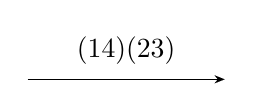
\begin{tikzpicture}
				\draw[-{Stealth[length=1.25mm, width=1mm]}, line width=0.01pt] (0,0) -- (2.5,0)
				node[midway, above=2pt] {$(14)(23)$};
			\end{tikzpicture}
		\end{center}
	\end{minipage}
	\begin{minipage}{0.56\textwidth}
		\begin{center}
			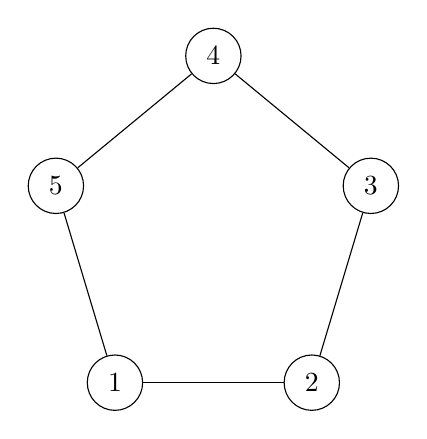
\begin{tikzpicture}
				\node[vertex] (a) at (2, 4.9) {$4$};
				\node[vertex] (b) at (4, 3.25) {$3$};
				\node[vertex] (c) at (3.25, 0.75) {$2$};
				\node[vertex] (d) at (0.75, 0.75) {$1$};
				\node[vertex] (e) at (0, 3.25) {$5$};

				\draw[edge] (a) to (b);
				\draw[edge] (b) to (c);
				\draw[edge] (c) to (d);
				\draw[edge] (d) to (e);
				\draw[edge] (e) to (a);
			\end{tikzpicture}
		\end{center}
	\end{minipage}

	\vspace{2em}

	which is evidently adjacency-preserving. Thus, $(14)(23) \in D_{5}$.
\end{solution}

\begin{subproblem}
	$(14)(35)$.
\end{subproblem}

\begin{solution}
	$(14)(35)$ doesn't belong to $D_{5}$. To see why, notice that $(14)(35)$ would permute the vertices of a pentagon like so:

	\vspace{2em}

	\begin{minipage}{0.40\textwidth}
		\begin{center}
			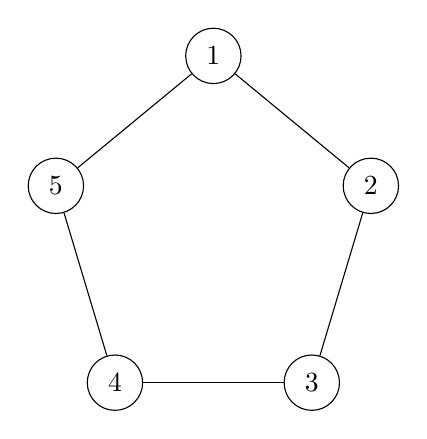
\begin{tikzpicture}
				\node[vertex] (a) at (2, 4.9) {$1$};
				\node[vertex] (b) at (4, 3.25) {$2$};
				\node[vertex] (c) at (3.25, 0.75) {$3$};
				\node[vertex] (d) at (0.75, 0.75) {$4$};
				\node[vertex] (e) at (0, 3.25) {$5$};
	
				\draw[edge] (a) to (b);
				\draw[edge] (b) to (c);
				\draw[edge] (c) to (d);
				\draw[edge] (d) to (e);
				\draw[edge] (e) to (a);
			\end{tikzpicture}
		\end{center}
	\end{minipage}
	\begin{minipage}{0.04\textwidth}
		\begin{center}
			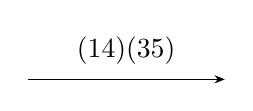
\begin{tikzpicture}
				\draw[-{Stealth[length=1.25mm, width=1mm]}, line width=0.01pt] (0,0) -- (2.5,0)
				node[midway, above=2pt] {$(14)(35)$};
			\end{tikzpicture}
		\end{center}
	\end{minipage}
	\begin{minipage}{0.56\textwidth}
		\begin{center}
			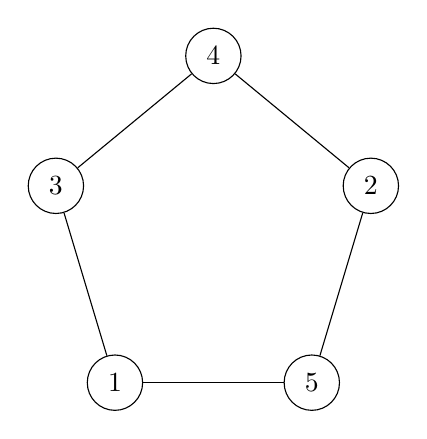
\begin{tikzpicture}
				\node[vertex] (a) at (2, 4.9) {$4$};
				\node[vertex] (b) at (4, 3.25) {$2$};
				\node[vertex] (c) at (3.25, 0.75) {$5$};
				\node[vertex] (d) at (0.75, 0.75) {$1$};
				\node[vertex] (e) at (0, 3.25) {$3$};

				\draw[edge] (a) to (b);
				\draw[edge] (b) to (c);
				\draw[edge] (c) to (d);
				\draw[edge] (d) to (e);
				\draw[edge] (e) to (a);
			\end{tikzpicture}
		\end{center}
	\end{minipage}

	\vspace{2em}

	which isn't adjacency preserving since, for example, $1$ becomes adjacent to vertex $3$ after the permutation, whereas that was not the case in the original pentagon. Thus, since $(14)(35)$ isn't an adjacency preserving permutation, it cannot belong to $D_{5}$.
\end{solution}





























\ifdefined\iscombined
	\newpage
\else
	\end{document}
\fi
